% Inspired by Dan Spielman's template

\documentclass[10pt]{article}
\usepackage[T1]{fontenc}
\usepackage{graphicx}

\usepackage{tikz}
\usetikzlibrary{arrows,matrix}
\usepackage{subfigure}
\usepackage{stackrel}
\usepackage{blindtext}
\usepackage{multicol}

\oddsidemargin=0.15in
\evensidemargin=0.15in
\topmargin=-.5in
\textheight=9in
\textwidth=6.25in

\usepackage[colorlinks=true,breaklinks,pdfpagemode=none,linkcolor=blue, urlcolor = blue, citecolor=blue]{hyperref}
\usepackage{enumerate}

%\usepackage{enumitem}
%\setlist{itemsep=0mm}

%\usepackage[usenames,dvipsnames]{pstricks}
%\usepackage{epsfig}
\usepackage{amsmath,amsfonts,amssymb,bm}
\usepackage[linesnumbered,ruled,vlined]{algorithm2e}
%\usepackage{pst-grad} % For gradients
%\usepackage{pst-plot} % For axes

% Enviroment definitions (add your own here)

\newtheorem{theorem}{Theorem}
\newtheorem{corollary}[theorem]{Corollary}
\newtheorem{lemma}[theorem]{Lemma}
\newtheorem{observation}[theorem]{Observation}
\newtheorem{proposition}[theorem]{Proposition}
\newtheorem{definition}[theorem]{Definition}
\newtheorem{claim}[theorem]{Claim}
\newtheorem{fact}[theorem]{Fact}

\newenvironment{proof}{\noindent{\bf Proof}\hspace*{1em}}{\qed\bigskip}

% New commands (add your own here)

\newcommand{\eps}{\varepsilon}
\newcommand{\bbR}{\mathbb{R}}
\newcommand{\hv}{\hat{v}}
\newcommand{\hL}{\hat{L}}
\newcommand{\hlambda}{\hat{\lambda}}
\newcommand{\homega}{\hat{\omega}}
\newcommand{\hp}{\hat{p}}
\newcommand{\hW}{\hat{W}}
\newcommand{\cK}{\mathcal{K}}
\newcommand{\qed}{\rule{7pt}{7pt}}
\newcommand{\cF}{\mathcal{F}}

\begin{document}

    \noindent
    \begin{center}

        \hrulefill

        \vspace{5pt}

        \makebox[\textwidth]{ {\bf AB IdeaLab, Competitive Programming Team, Fall 18--Spring 19} \hfill  February 8, 2019}
        \vspace{0pt}

        {\Large \hfill  Lecture 2: Data Structures\hfill}
        \vspace{10pt}

        {\large \hfill  American Computer Science League, February Contest\hfill}
        \vspace{10pt}

        \makebox[\textwidth]{ {\it Lecturer: Sanjit Bhat \hfill Editor: Alexander Sun} } % primary editor is the 'lecturer'

        \vspace{-3pt}
        \hrulefill
    \end{center}

\section{Introduction}
In the modern era where data is being produced at a rapidly increasing
pace\footnote{With the Internet of Things, everything from a lightbulb
to your car is generating data.}
and being used for ever-increasing
applications\footnote{With Machine Learning, data-driven services like Google Translate and
FaceID reach billions of users each day},
we need fast ways of storing data.
Ideally, we could develop one data structure to hold all types of data
and perform all operations in the quickest time possible, however,
such a structure is currently nonexistent.
Instead, computer scientists need to be able to determine what
data structures to use in their specific problem.

For the purposes of ACSL, we will be studying four data structures
in the following lecture: stacks, queues, binary search trees, and
heaps/priority queues.
We will go through what each of them are, how they operate,
operations you can do on them, and the runtime complexity for each operation.
Hopefully, you will find the complexity analysis to be an interesting intellectual endeavor.
If not, you will end up seeing this stuff a lot more in intermediate--advanced CS
classes in college and in job interviews, so it's a good idea to start learning them now.

\paragraph{Basics on runtime.}
For the following analyses, we will be making use of Big(O) notation.
If you don't understand what expressions like $\mathcal{O}(n\log{}n)$ mean,
read \href{https://www.topcoder.com/blog/learning-understanding-big-o-notation/}{this Topoder article}
for a brief introduction.

\section{Stacks}
A good mental model for a stack is to picture a stack of books.
You start the school year by putting the Resnick and Halliday AP Physics
textbook down, but you never touch it after.
Eventually, after the AP is done and McClung or Bradford asks for the textbook,
you go to search for it.
However, since it is now under a pile of 5 other textbooks, it takes a lot of effort to pull out.

The book stack here works in exactly the same way as a stack data structure.
It follows a ``Last-In, First-Out'' (LIFO) ordering, which means that the objects
put in last come out first.
In the textbook example, while it takes a lot of effort to pull out your physics textbook,
your stats textbook (which you just put in yesterday) slides right off the top.

A visual representation of a stack follows.
To sum up what we've been discussing, it is clear how incoming objects
get placed on the top of the list, which is the same place where
objects are removed.
\begin{center}
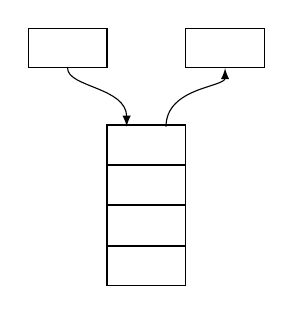
\begin{tikzpicture}[draw, minimum width=1cm, minimum height=0.5cm]
    \node[draw] (in) at (-1,2) {};
    \node[draw] (out) at (1,2) {};
    \matrix (queue)[matrix of nodes, nodes={draw, nodes={draw}}, nodes in empty cells]
    {
       \\ \\ \\ \\
    };

    \draw[-latex] (0.25,1) .. controls (0.25,1.5) and (1,1.5) .. (out.south);
    \draw[-latex] (in.south) .. controls (-1, 1.5) and (-0.25,1.5) .. (-0.25,1);
\end{tikzpicture}
\end{center}

For ACSL, we will be given one of two commands: PUSH(element) or X = POP().
PUSH pushes an element to the top of the stack, while POP removes the top element
and assigns it to some variable.
If the stack is empty, POP returns NIL\@.

\section{Queues}
Similar to stacks, queues have the exact same list representation and the exact
same operations, PUSH and POP\@.
However, while stacks pop from the top of the list, queues pop from the bottom.
In other words, queues have ``First-In, First-Out'' (FIFO) ordering.

A nice mental model for FIFO queues can be seen through the order line
in a fast-food restaurant.
As customers enter, they must wait till they reach the front until they can order.
Once at the front, out of all the people in the queue,
they are the first ones chronologically (First-In) who entered
and the first ones out (First-Out).
The following diagram sums everything up.
Notice how we still add new items to the top.
We just remove items from the bottom.
\begin{center}
\begin{tikzpicture}[draw, minimum width=1cm, minimum height=0.5cm]
    \node[draw] (in) at (-1,2) {};
    \node[draw] (out) at (1,-2) {};
    \matrix (queue)[matrix of nodes, nodes={draw, nodes={draw}}, nodes in empty cells]
    {
       \\ \\ \\ \\
    };

    \draw[-latex] (0.25,-1) .. controls (0.25,-1.25) and (1,-1.25) .. (out.north);
    \draw[-latex] (in.south) .. controls (-1, 1.5) and (-0.25,1.5) .. (-0.25,1);
\end{tikzpicture}
\end{center}

\paragraph{Sample problem.} What are the values popped and the items remaining
on the list if the following commands are applied to a stack and queue:
\begin{multicols}{4}
\begin{enumerate}
\item PUSH(``A'')
\item PUSH(``M'')
\item PUSH(``E'')
\item X = POP()
\item PUSH(``R'')
\item X = POP()
\item PUSH(``I'')
\item X = POP()
\item X = POP()
\item X = POP()
\item X = POP()
\item PUSH(``C'')
\item PUSH(``A'')
\item PUSH(``N'')
\end{enumerate}
\end{multicols}

Answer: For a stack, the values popped are E, R, I, M, A, and NIL.
The items remaining will be N and C, with N at the top.
For a queue, the values popped are A, M, E, R, I, and NIL.
The items remaining will be N, A, and C, with N at the top.

\paragraph{A note on runtimes.}
Both stacks and queues use Linked Lists as their underlying representations.
For stacks, we store a reference to the top.
For queues, we store references to both the top and bottom.
Thus, when we want to push or pop, we just access the references directly,
which is an $\mathcal{O}(1)$ operation.


\section{Binary search trees}
This is where shit gets interesting\ldots
 A binary search tree (BST) consists of several nodes arranged in a tree-like
structure (i.e., with nodes branching off of other nodes).
The following is a diagram for the BST of \{Java, Python, C++, JavaScript,
LISP, Assembly, Fortran\} (in that order),
which will will help me explain some important information:
\begin{center}
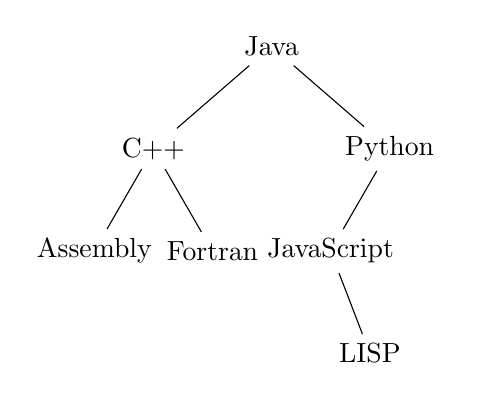
\begin{tikzpicture}[level distance=1.3cm,
    level/.style = {sibling distance = 30mm/#1}]
\node {Java}
   child {node {C++}
       child {node {Assembly}}
       child {node {Fortran}}
    }
    child {node {Python}
        child {node {JavaScript}
            child {edge from parent[draw = none]}
            child {node {LISP}}}
        child {edge from parent[draw = none]}
    };
\end{tikzpicture}
\end{center}

\begin{enumerate}
\item \textit{Root node.}
The root node forms the top of the tree.
In this example, the root node is labeled ``Java.''

\item \textit{Child node.}
Every node can have zero, one, or two children (nodes directly coming out
of it).
In the above diagram, the root node has ``C++'' and ``Python'' as its children.

\item \textit{Ordering.}
The BST is arranged in a particular structure.
Namely, the left child of any node needs to have a value that is less than or equal
to that node.
The right child needs to have a value that is strictly greater than that node.

\item \textit{Depth.}
The root node is defined to have a depth of 0.
Every subsequent node has a depth that is equal to how far away it is
from the root node.
For example, ``C++'' and ``Python'' have depth 1, while ``LISP'' has depth 3.

\item \textit{Leaf node.}
A leaf node is the most lonely node---it has no children.
Here, ``Assembly,'' ``Fortran,'' and ``LISP'' are leaf nodes (which is quite
inaccurate to reality since they pioneered several offspring languages).

\item \textit{Internal nodes.}
The set of nodes currently in the BST, \{Java, Python, C++, JavaScript,
LISP, Assembly, Fortran\}.

\item \textit{Internal path length.}
The sum of the depths of the internal nodes, 0 + 1 + 1 + 2 + 3 + 2 + 2 = 11.

\item \textit{External nodes.}
The set of nodes that could possibly be attached to the BST.
I will demarcate these nodes with a ``?'' in the following diagram.
\begin{center}
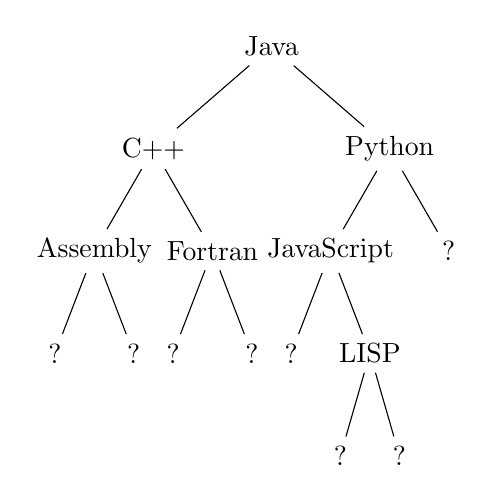
\begin{tikzpicture}[level distance=1.3cm,
    level/.style = {sibling distance = 30mm/#1}]
\node {Java}
    child {node {C++}
        child {node {Assembly}
            child {node {?}}
            child {node {?}}}
        child {node {Fortran}
            child {node {?}}
            child {node {?}}}
    }
    child {node {Python}
        child {node {JavaScript}
            child {node {?}}
            child {node {LISP}
                child {node {?}}
                child {node {?}}}}
        child {node {?}}
    };
\end{tikzpicture}
\end{center}

\item \textit{External path length.}
The sum of the depths of the hypothetical, external nodes,
3 + 3 + 3 + 3 + 3 + 4 + 4 + 2 = 25.
Note that the external path length can be calculated through the following formula:
\begin{equation*}
(\text{internal path length}) + 2 * (\text{number of internal nodes}).
\end{equation*}
In this case, the formula would give 11 + 2 * 7 = 25.
We ran out of time to prove this in the 2018--19 season, so this remains
an unsolved problem for future CPT members.
\end{enumerate}

\paragraph{BST traversal.}
Traversal problems often ask for the order you would reach every single node
given a certain traversal method.
For the purposes of ACSL, there are three traversal methods for a BST:
inorder, preorder, and postorder.
Each refers to the order of traversal of the current node relative to the
left and right nodes (e.g., inorder traverses left, current, right;
preorder traverses current, left, right;
and postorder traverses left, right, current).
Given a specific traversal order, our method of determining which nodes
come first will henceforth be called the \textit{Jelinsky Method}.

The Jelinsky Method proceeds as follows:
\begin{itemize}
\item We write the traversal order of the Left child, the Right child,
and the current node, as defined by the given traversal method.
\item We cross off
the next available letter and move in that corresponding direction.
\item When we run out of letters, we move
back up to that node's parent.
\item When we cross off the C, we have ``visited'' the current node
and add it to our list of visited nodes.
\end{itemize}

As a demonstration for the prior BST, let's assume we want to traverse in postorder.
We write L, R, C next to every node and start from the root.
We cross the L off of ``Java'' and move to its left child, ``C++''.
We cross off the L in ``C++'' and move to ``Assembly''.
We cross off the L and R in ``Assembly'' and try to move to its left and right children,
but since no such children exist, we stay at ``Assembly''.
We cross off the C in ``Assembly'' and add it to our list of visited nodes.
Thus, using postorder traversal, we arrive at ``Assembly'' first.

Next, since we have crossed off the L, R, and C in ``Assembly,''
we move back up to its parent, ``C++''.
We have already crossed off the L in ``C++,'' so we cross off the R and move
into ``Fortran.''
As you can imagine, this process keeps on going until we have traversed
the entire tree.
Overall, our traversal order would be \{Assembly, Fortran, C++, LISP,
Javascript, Python, Java\}.

\paragraph{Searching for and inserting nodes into a BST.}
The algorithms for searching and inserting into a BST are nearly identical:
they both proceed down the tree comparing a given value to the nodes of the tree.
Specifically, we start from the root node and do the following:
\begin{itemize}
\item If the given value is \textbf{less than or equal to} the current node, move
to the left child.
\item If the given value is greater than the current node, move to the right child.
\item Keep on iterating until the value is either found (searching) or
until you arrive at a place to add the node (inserting).
\end{itemize}

What's important about both of the above functions is that they use
the BST's implicit ordering of the children relative to the parent node.
This enables them to perform a maximum of $d$ comparison operations,
where $d$ is the BST's depth.
For a well-balanced tree (i.e., the nodes are not stacked
on one side of the tree), $d$ is approximately equal to the log base 2
of the number of nodes.
This makes the running time $\mathcal{O}(\log{}n)$, where $n$ is the number
of nodes.

\paragraph{Removing a node.}
Removing is slightly more complex.
To remove a node $p$, we first use the searching algorithm above to find it.
Then, if $p$ has no children, we simply remove it.
If it has one child, we make $p$'s child become $p$'s parent's child.

The case where $p$ has two children is the most complex:
since both children could possibly have children of their own, we need to be careful.
First, we make an arbitrary decision to make $p$'s left child become $p$'s parent's child.
Then, we keep on moving the right branch of $p$ down the left child's branch until we
arrive at the highest node (the node furthest right) in the left branch.
We know that every node in the original right branch is greater than this node,
so we simply add the right branch as the right child of this node.

\section{Heaps and priority queues}
\paragraph{Motivating discussion.}
There are several applications where we want to find the smallest (or largest) node in a set.
For example, let's say we are trying to drive from place A to place B
in the shortest amount of time.
We come up with estimates for the time it would take through different routes,
and we constantly determine the minimum current
estimate and perform updates to our estimates using new
information\footnote{Such a process is used in Dijkstra's Algorithm}.
In this case, both BSTs and Heaps
provide $\mathcal{O}(\log{}n)$ updates,
but Heaps let you determine the minimum current estimate in $\mathcal{O}(1)$
as opposed to $\mathcal{O}(\log{}n)$.
To say it plainly, Heaps allow for really quick determination of the
minimum element in your set.

\paragraph{Structure.}
Heaps (also called Priority Queues) are fundamentally tree-like.
Compared to BST's ``Left-lesser, Right-greater'' ordering, however, they
enforce that every child (irrespective of left or right)
has a value greater than that of the current node.
This allows them to access the minimum node in $\mathcal{O}(1)$ time.
An example HEAP follows, built using the letters \{A, M, E, R, I, C, A, N\}
(in that order).
\begin{center}
\begin{tikzpicture}[level distance=1.3cm,
    level/.style = {sibling distance = 30mm/#1}]
\node {A}
    child {node {I}
        child {node {N}
            child {node {R}}
            child {edge from parent[draw = none]}}
        child {node {M}}
    }
    child {node {A}
        child {node {E}}
        child {node {C}}
    };
\end{tikzpicture}
\end{center}

Compared to BSTs, you may notice that the above Heap looks more completely filled.
This is purposeful.
Every level in the tree except the bottom-most level is completely filled.
To add a new node, we go to the bottom-most level and fill from left to right.
The completely filled nature of Heaps gets rid of some of the
balancing problems of BSTs and ensures the depth $d$
will always be the log base 2 of the number of nodes.

\paragraph{Inserting a new node.}
As mentioned above, we first insert a node in the deepest tree level from left to right.
After insertion at the bottom, we ``bubble'' up, switching the node with its
parent if it has a smaller value.
Since the other child node is guaranteed to have a larger value than the
parent (which in turn has a larger value than the inserted node),
the Heap's ordering is preserved under ``bubbling''.
Moreover, since our number of switches is at max the depth $d$ of our tree,
insertion is $\mathcal{O}(\log{}n)$!

This is what the above Heap would look like if we added the character C.
Trace out the bubbling yourself to make sure you understand the process.
\begin{center}
\begin{tikzpicture}[level distance=1.3cm,
    level/.style = {sibling distance = 30mm/#1}]
\node {A}
    child {node {C}
        child {node {I}
            child {node {R}}
            child {node {N}}}
        child {node {M}}
    }
    child {node {A}
        child {node {E}}
        child {node {C}}
    };
\end{tikzpicture}
\end{center}

\paragraph{Deleting the root node.}
To delete the root node, we switch it with the bottom-most and right-most node
and delete the old root.
Then, instead of bubbling up, we bubble \textit{down} from the new root node (previously
one of the largest nodes),
switching with the smaller of the two child nodes.
This specific switch ensures that the other child node is still larger
than its new parent node and that the Heap ordering is preserved.
In addition, since we only have to perform $d$ bubble downs,
deleting the root node is $\mathcal{O}(\log{}n)$.

What follows is the result of deleting the root node from our updated Heap.
\begin{center}
\begin{tikzpicture}[level distance=1.3cm,
    level/.style = {sibling distance = 30mm/#1}]
\node {A}
    child {node {C}
        child {node {I}
            child {node {R}}
            child {edge from parent[draw = none]}}
        child {node {M}}
    }
    child {node {C}
        child {node {E}}
        child {node {N}}
    };
\end{tikzpicture}
\end{center}

\paragraph{Critical thinking.}
In a min-heap (i.e., where the root node is the minimum element),
what is the time complexity for finding the maximum element?

First, observe that since the children of a particular node will always
be larger than it, we can find the node in the last level of the Heap.
Moreover, compared to a BST where we would need to traverse all the way down the
tree to get to the final level,
we usually store Heaps in arrays due to their sequential and predictable algorithm
for insertion and deletion.
This enables us to look at the last few elements of the array to find the last level
of the tree.

However, it isn't all well and good for Heaps.
Since the number of nodes in the last layer is approximately equal to $n/2$, where
$n$ is the number of nodes, the time complexity would still be $\mathcal{O}(n/2)$,
which reduces to $\mathcal{O}(n)$.
This points to one of the disadvantages of Heaps.
Compared to the more versatile BST which can find the minimum and maximum
elements in $\mathcal{O}(\log{}n)$,
Heaps are much more specialized.
They perform some operations (e.g., finding the minimum value)
in constant time, but take much more time for other operations compared to BSTs.

\section{Exercises}
\begin{enumerate}
\item When ``Grumpy'' is inserted into the following binary search tree, what
is the new external path length of the tree?
\begin{center}
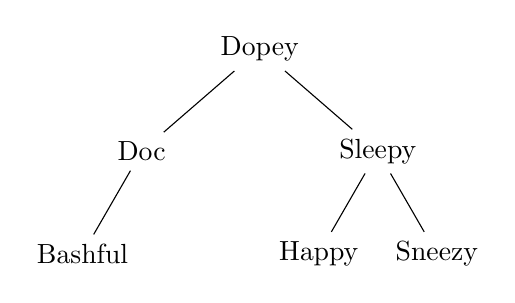
\begin{tikzpicture}[level distance=1.3cm,
level/.style = {sibling distance = 30mm/#1}]
\node {Dopey}
   child {node {Doc}
       child {node {Bashful}}
       child {edge from parent[draw = none]}
       }
    child {node {Sleepy}
       child {node {Happy}}
       child {node {Sneezy}}
       };
\end{tikzpicture}
\end{center}

\item Consider the following operations on an initially empty stack.
If a POP is now performed, what value would be popped?
\begin{multicols}{4}
\begin{enumerate}
\item PUSH(``B'')
\item PUSH(``I'')
\item PUSH(``N'')
\item X = POP()
\item PUSH(``D'')
\item X = POP()
\item PUSH(``S'')
\item X = POP()
\end{enumerate}
\end{multicols}

\item Consider an initially empty stack.
After the following operations are performed, what is the value of Z?
\begin{multicols}{3}
\begin{enumerate}
\item PUSH(3)
\item PUSH(6)
\item PUSH(8)
\item Y = POP()
\item X = POP()
\item PUSH(X - Y)
\item Z = POP()
\end{enumerate}
\end{multicols}

\item Create a min-heap with the letters in the word PROGRAMMING.
What are the letters in the bottom-most row, from left to right?

\item Create a binary search tree from the letters in the word PROGRAM.
What is the internal path length?

\item Which of the following binary trees are valid binary search trees?

\begin{multicols}{3}
\begin{enumerate}
\item
\begin{tikzpicture}[level distance=1.3cm,
level/.style = {sibling distance = 30mm/#1}]
\node {A}
    child {edge from parent [draw = none]}
    child {node {C}
        child {edge from parent [draw = none]}
        child {node {S}
            child {node {L}}
            child {edge from parent [draw = none]}}
    };
\end{tikzpicture}

\item
\begin{tikzpicture}[level distance=1.3cm,
level/.style = {sibling distance = 30mm/#1}]
\node {J}
    child {node {B}}
    child {node {S}
        child {node {R}}
        child {node {T}}
    };
\end{tikzpicture}

\item
\begin{tikzpicture}[level distance=1.3cm,
level/.style = {sibling distance = 30mm/#1}]
\node {B}
    child {edge from parent [draw = none]}
    child {node {R}
        child {node {O}
            child {edge from parent [draw = none]}
            child {node {W}
                child {node {N}}
                child {edge from parent [draw = none]}}}
        child {edge from parent [draw = none]}
    };
\end{tikzpicture}

\item
\begin{tikzpicture}[level distance=1.3cm,
level/.style = {sibling distance = 30mm/#1}]
\node {A}
    child {edge from parent [draw = none]}
    child {node {W}
        child {node {F}
            child {edge from parent [draw = none]}
            child {node {T}
                child {node {M}}
                child {edge from parent [draw = none]}}}
        child {edge from parent [draw = none]}
    };
\end{tikzpicture}

\item
\begin{tikzpicture}[level distance=1.3cm,
level/.style = {sibling distance = 30mm/#1}]
\node {S}
    child {node {A}}
    child {node {Z}
        child {node {M}}
        child {node {Q}}
    };
\end{tikzpicture}
\end{enumerate}
\end{multicols}

\item If one traversed the following tree in preorder, in what order would nodes
be visited?
Be sure your answer is neat and clear!
\begin{center}
\begin{tikzpicture}[level distance=1.3cm,
level/.style = {sibling distance = 30mm/#1}]
\node {A}
    child {node {B}
        child {node {D}}
        child {node {E}}
        child {node {F}
            child {node {H}}
            child {node {I}}}}
    child {node {C}
        child {node {G}}
    };
\end{tikzpicture}
\end{center}

\end{enumerate}

\newpage
\section{Solutions}
\begin{enumerate}
\item 25

\item ``I''

\item -2

\item Here is the min-heap.
As can be seen, the bottom row contains the letters R, O, R, and N.
\begin{center}
\begin{tikzpicture}[level distance=1.3cm,
    level/.style = {sibling distance = 30mm/#1}]
\node {A}
    child {node {G}
        child {node {M}
            child {node {R}}
            child {node {O}}}
        child {node {I}
            child {node {R}}
            child {node {N}}}
    }
    child {node {G}
        child {node {P}}
        child {node {M}}
    };
\end{tikzpicture}
\end{center}

\item What follows is the BST.
The internal path length is 0 + 1 + 1 + 2 + 2 + 3 + 3 = 12.
\begin{center}
\begin{tikzpicture}[level distance=1.3cm,
    level/.style = {sibling distance = 30mm/#1}]
\node {P}
    child {node {O}
        child {node {G}
            child {node {A}}
            child {node {M}}}
        child {edge from parent[draw = none]}
    }
    child {node {R}
        child {node {R}}
        child {edge from parent[draw = none]}
    };
\end{tikzpicture}
\end{center}

\item Recall the ``Left-lesser, Right-greater'' ordering of BSTs.
Using that, we get (a), (b), and (d).

\item Trees are not just limited to having 2 nodes!
The answer here is A, B, D, E, F, H, I, C, G, A.
\end{enumerate}

%\begin{thebibliography}{9}
%    \bibitem{deep_learning}
%    Lecun, Y., Bengio, Y., and Hinton, G. (2015).
%    Deep learning.
%    Nature, 521(7553), 436-444.
%\end{thebibliography}
\end{document}